\begin{frame}{Function Selection}
Important genomics task: Identify interdependent effect of mutations. \\
\vspace{0.1in}
$\func$ has $50$ variables, but true interactions are pairwise (or
low order) and sparse.
\[
f(x_1^{50}) = f(x_2,x_7) + f(x_{21},x_{34}) + \dots + f(x_{12},x_{49})
\]
4/50 individual effects and 4/1225 pairwise effects \\
\centering
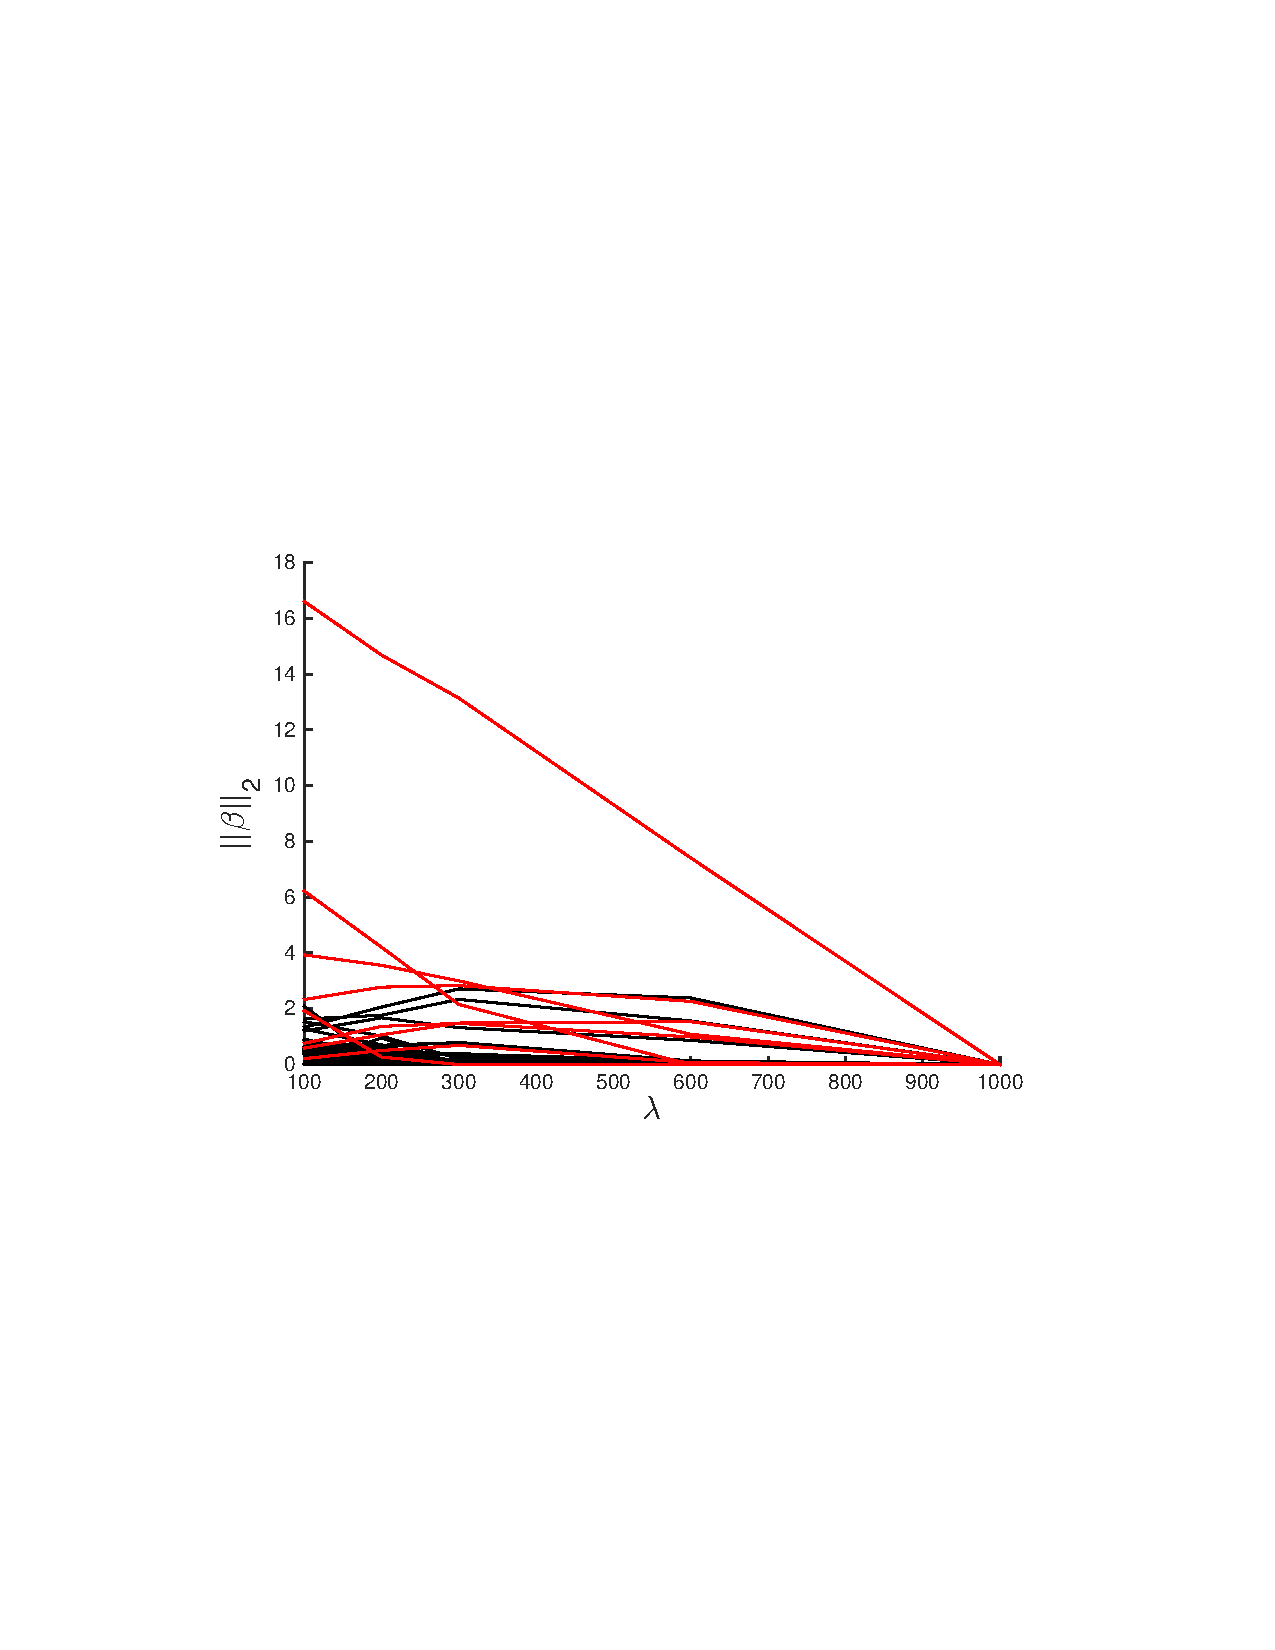
\includegraphics[width=0.5\textwidth]{figs/solnpath600.pdf} \\
Recovers all true nonzero functions with FPR=3.7\%
\end{frame}

\begin{frame}{Optimization Problem}
Recall objective:  $\alphaj \in \RR^n$, $\aalpha \in \RR^{nM}$
\begin{equation*}
\min_\aalpha \frac{1}{2}\Big\|Y - \sum_{j=1}^m \KKj \alphaj\Big\|_2^2 + 
  \lambda \sum_{j=1}^M \sqrt{{\alphaj}^\top \KKj \alphaj}
\end{equation*} \\
\begin{itemize}
\item  Challenge: generalized sum-of-norms regularization:
\begin{equation*}
\sqrt{{\alphaj}^\top \KKj \alphaj} = \|{R^{(j)}} \alphaj \|_2 
\text{ where } \KKj = {R^{(j)}}^\top {R^{(j)}}
\end{equation*}
\end{itemize}
Rewrite with Cholesky decomposition: $\KKj = \LLj \LLj^\top$. \\ 
Let $\betaj = \LLj^\top \alphaj$
\begin{equation*}
\min_{\bbeta \in \RR^{nM}} 
\frac{1}{2}\Big\|Y - \sum_{j=1}^m \LLj \alphaj\Big\|_2^2 + 
\lambda \sum_{j=1}^M \|\betaj\|_2
\end{equation*}
\vspace{-0.2in}
\begin{itemize}
\item Group lasso problem!
\end{itemize}
\end{frame}

\begin{frame}{Optimization methods}
\begin{itemize}
\item Subgradient / Proximal gradient: iteration cost $O(n^2M)$
\item ADMM: medium convergence, iteration cost $O(n^2M^2)$ \\
Main cost: solve triangular $nM \times nM$ system in primal update
\item Exact BCD: fast convergence, iteration cost $O(n^3 M)$ \\
\begin{itemize}
\item Quickly solve 1d problem for $\Delta$
$\|-(\Delta \LLjt\LLj + \lambda I)^{-1}(\LLjt (\sum_{i\neq j}\LLi \betai))\|=1$
\item Then solve $n \times n$ system for 
$\betaj \leftarrow -(\Delta \LLjt\LLj+\lambda I)^{-1}(\LLjt(\sum_{i\neq j}\LLi \betai))/\Delta$
\end{itemize}
\item BCGD: medium convergence, iteration cost $O((n^2+nM)M)$
\begin{itemize}
\item Block coordinate gradient descent (Tseng \& Yun, 2007) 
with diagonal Hessian approximation
\item Backtracking is relatively expensive, so we skip
\end{itemize}
\end{itemize}
\end{frame}

\begin{frame}{Optimization results}
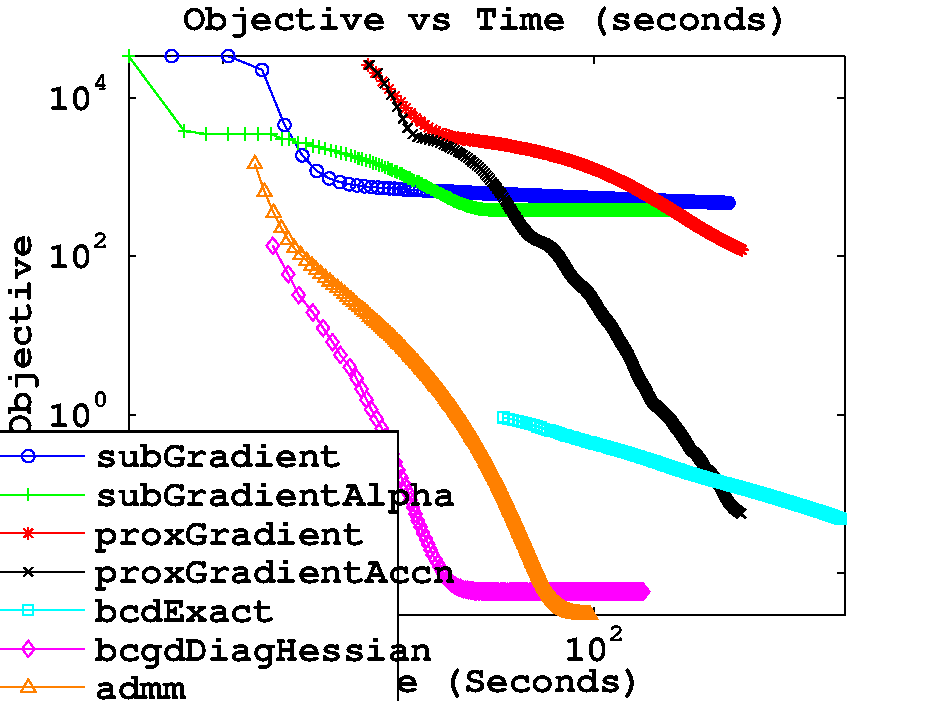
\includegraphics[width=\textwidth]{figs/time1000v2.eps}
\end{frame}
